\documentclass[tikz,border=6pt]{standalone}
\usepackage{amsmath,amssymb}
\usepackage{tikz}
\usetikzlibrary{arrows.meta}

\begin{document}
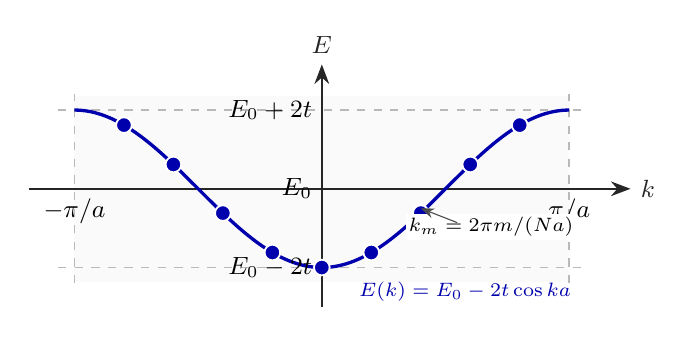
\begin{tikzpicture}[
  >=Stealth,
  axis/.style={->, line width=0.9pt, black!85},
  guide/.style={dashed, gray!55, line width=0.55pt},
  curve/.style={very thick, blue!68!black},
  filled allowed/.style={circle, draw=white, fill=blue!68!black, line width=0.65pt, inner sep=2pt},
  every node/.style={font=\small}
]
  % Vertical coordinate is E-E_0 in units of 2t.
  \fill[gray!4] (-3.14159,-1.18) rectangle (3.14159,1.18);
  \draw[axis] (-3.72,0) -- (3.92,0) node[right] {$k$};
  \draw[axis] (0,-1.5) -- (0,1.58) node[above] {$E$};

  \draw[guide] (-3.14159,-1.2) -- (-3.14159,1.2);
  \draw[guide] (3.14159,-1.2) -- (3.14159,1.2);
  \draw[guide] (-3.35,1) -- (3.35,1);
  \draw[guide] (-3.35,-1) -- (3.35,-1);

  \draw[curve, domain=-3.14159:3.14159, samples=200]
    plot (\x, {-cos(\x r)});

  \foreach \x in {-2.513,-1.885,-1.257,-0.628,0,0.628,1.257,1.885,2.513} {
    \node[filled allowed] at (\x, {-cos(\x r)}) {};
  }

  \node[below] at (-3.14159,0) {$-\pi/a$};
  \node[below] at (3.14159,0) {$\pi/a$};
  \node[left] at (0,1) {$E_0+2t$};
  \node[left] at (0,0) {$E_0$};
  \node[left] at (0,-1) {$E_0-2t$};
  \node[blue!68!black, font=\scriptsize, below right] at (0.35,-1.06) {$E(k)=E_0-2t\cos ka$};
  \node[font=\scriptsize, fill=white, inner sep=1.2pt] at (2.15,-0.48) {$k_m=2\pi m/(Na)$};
  \draw[->, thin, black!70] (1.72,-0.43) -- (1.257,{-cos(1.257 r)+0.06});
\end{tikzpicture}
\end{document}
